\documentclass{scsSimAUDPaperFormat}
% Beginning of preable.
% Ensure that the copyright notice matches the conference/symposium.
\copyrightnotice{
	SimAUD 2020 May 25-27 Vienna, Austria
	
	\copyright\,2020 Society for Modeling \& Simulation International (SCS)
}
% Load basic packages
\usepackage{balance}		% to better equalize the last page
\usepackage{graphics}		% for EPS, load graphicx instead
\usepackage{times}			% comment if you want LaTeX's default font
\usepackage{url}			% llt: nicely formatted URLs
\usepackage{dblfloatfix}	% allow placement of a page-width figure at top or bottom of page
% llt: Define a global style for URLs, rather that the default one

\usepackage{listings}
\lstdefinestyle{mystyle}{
    %backgroundcolor=\color{backcolour},   
    %commentstyle=\color{codegreen},
    keywordstyle=\color{magenta},
    %numberstyle=\tiny\color{codegray},
    %stringstyle=\color{codepurple},
    basicstyle=\ttfamily\footnotesize,
    breakatwhitespace=false,         
    breaklines=true,                 
    captionpos=b,                    
    keepspaces=true,                 
    numbers=left,                    
    numbersep=5pt,                  
    showspaces=false,                
    showstringspaces=false,
    showtabs=false,                  
    tabsize=2
}
 
\lstset{style=mystyle}

\makeatletter
\def\url@leostyle{%
  \@ifundefined{selectfont}{\def\UrlFont{\sf}}{\def\UrlFont{\small\bf\ttfamily}}}
\makeatother
\urlstyle{leo}

% To make various LaTeX processors do the right thing with page size.
\def\pprw{8.5in}
\def\pprh{11in}
\special{papersize=\pprw,\pprh}
\setlength{\paperwidth}{\pprw}
\setlength{\paperheight}{\pprh}
\setlength{\pdfpagewidth}{\pprw}
\setlength{\pdfpageheight}{\pprh}

% Make sure hyperref comes last of your loaded packages,
% to give it a fighting chance of not being over-written,
% since its job is to redefine many LaTeX commands.
\usepackage[pdftex]{hyperref}
\hypersetup{
pdftitle={SCS Conference Proceedings Format},
pdfauthor={LaTeX},
pdfkeywords={SCS, proceedings, archival format},
bookmarksnumbered,
pdfstartview={FitH},
colorlinks,
citecolor=black,
filecolor=black,
linkcolor=black,
urlcolor=black,
breaklinks=true,
}

% create a shortcut to typeset table headings
\newcommand\tabhead[1]{\small\textbf{#1}}

% create an affilitation superscript
\newcommand{\affiliation}[1]{\ensuremath{^{\textrm{#1}}}}

% End of preamble. Here comes the document.
\usepackage{verbatim}
\begin{document}
\title{
\includegraphics[width=1.0\textwidth]{SimAUDLogo.png}\\\quad\\Modeling and Simulation of Municipal Solid Waste Management System based on Discrete Event System Specification}

% Replace "UniversityA", "CompanyA", "UniversityB" with institution-specific abbreviations.
\def\UniversityA{\affiliation{1}} 
\def\CompanyA{\affiliation{2}}

\author{
	Chang-Hyun Lyoo\UniversityA
	,
	Jinho Jung\UniversityA
	,
	Changbeom Choi\UniversityA
	\,and
	Eun-Young Kim\CompanyA
	\\
	\\
\affaddr{\UniversityA}{Handong Global University, Pohang, Rep. of Korea, \{21300259, 21300704, cbchoi\}@handong.edu}\\
\affaddr{\CompanyA}{Pohang TechnoPark, Pohang, Rep. of Korea, hellosally@daum.net}
}

\maketitle

\begin{abstract}
%생활쓰레기수거는 시민들의 편의에 큰 영향을 미치는 중요한 도시행정서비스이다. 
The cleanliness of the residential area is one of the critical considerations for urban planning.~Especially, municipal waste management is a vital service that affects the resident's satisfaction level.~Since the satisfaction level may be affected by the amount of garbage accumulated at the time the residents discharge garbage, an urban planner may take an account of the resident's life pattern to build efficient waste collection strategy.~As the composition of residents in a residential area becomes complicated, estimating the accumulation of garbage based on the life patterns of residents is a difficult problem for urban planners to achieve the resident's high satisfaction level with the public service.~This research focuses on representing the temporal behavior pattern of residents in an area as a discrete event system.~Also, this research introduces a simulation environment which utilizes the discrete event system specification formalism to simulate the life pattern of residents and analyze waste generation and the municipal waste management system.~The simulation results show that modeling the life patterns and the housing types of the residents may represent the dynamics of the waste management system.

\end{abstract}

\keywords{
	Agent-based Simulation; Discrete Event System Formalism; Municipal Solid Waste Management System.
\\
}

% ACM Classification Keywords
\category{I.6.5} \
SIMULATION AND MODELING (Model Development).\\

\section{Introduction}
Today, almost 55\% of the world population lives in urban areas, and the population of the urban area keeps increasing~\cite{united20182018}. Among many urban issues, the garbage problem is most closely related to the satisfaction of citizens~\cite{mohit2010assessment}. As the population increases, the total amount of garbage within a local area may increase. Thereby, the satisfaction level of a resident may decrease when the Government does not collect the trash on time.  Also, unsatisfied citizens may compile civil complaints, and it leads to increasing the load of Government employees and the social cost.As a result, the urban planners or the employees of the Local Government analyze the residential area to estimate the amount of waste generation and provide appropriate public services to the city, such as utilizing garbage trucks to collect wastes. Despite these efforts, it is difficult to estimate the waste discharge pattern because the behavior patterns of residents are more important than considering the geographic or demographic characteristics of the residential area. Notably, residents' life patterns may differ to the cultural characteristics and occupational characteristics of a resident, so that considering the life patterns are a difficult problem. 

This research proposes a modeling method focusing on human characteristics and behavior patterns to help optimize municipal waste management systems. Since the temporal behavior of the residents may differ based on their life cycle and occupation, this research utilizes the Discrete Event System Specification(DEVS) formalism to model the behavior of the residents. The DEVS formalism is a set-theoretical framework and has a modular characteristic~\cite{Zeigler84, Zeigler90, tms2000}. Therefore, the simulationists may develop their simulation model as a component of the urban system or may reuse a different simulation model which is built by other simulationists.~To maximize the modular characteristic of the DEVS formalism, this research proposes an object-oriented discrete event simulator using the Python programming language.~The simulator captures the common behavior of the residents of the urban area using DEVS formalism and specializes in analyzing the residents by their occupation. Therefore, simulationists may reuse the DEVS simulation model to simulate the temporal behavior of the residents and may differentiate each resident by using occupation objects.

\section{Related Works and Backgrounds}
This section introduces the related works and analyzes them.~Also, it provides the background knowledge to help understanding the proposed method and the simulation environment.

\subsection{Related Works: Waste Management}
There have been many studies to optimize waste management by applying analytic solution and simulation technique. Dao Tuan et al. (2017) used Integer Linear Programming (ILP) and Mixed ILP to optimize the route of the garbage trucks considering emission control~\cite{dao2017optimizing}.

Some work has been done to optimize the route of the garbage trucks and reduce waste collection costs using agent-based simulation and GIS. Chalkias et al. (2009) have constructed spatial geo-database integrating GIS and municipality database~\cite{chalkias2009gis}. They have proposed an optimal path of garbage truck using Dijkstra's algorithm. Das et al. (2015) solved the waste transportation problem by optimizing the waste collection and transportation path with the aid of traveling salesman problem to develop time and cost-effective waste management system design, ~\cite{das2015optimization}. Nambiar et al. (2013) compared the static vehicle routing problem and dynamic vehicle routing problem and focused on increasing the capacity utilization of each participating vehicle~\cite{nambiar2013multi}. Nguyen et al. (2013) have proposed a model to optimize the collection and transportation of municipal solid waste, in terms of fuel consumption and pollutant emissions~\cite{nguyenemission}. Shi et al. have combined agent-discrete modeling techniques and Voronoi-based genetic algorithm and $k^{th}$ nearest search algorithm to build an optimization model~\cite{shi2013multi}. Also, they recommended vehicle routing and resource allocation for solid waste management systems. Karadimas et al. (2006) have suggested the loose coupling of GIS and simulation software in the municipal waste management area~\cite{karadimas2006coupling}. Hua et al. (2016) have proposed that applying GIS and real-time data of waste from smart devices to routing problems would reduce the traveling distance of vehicles~\cite{hua2016towards}.
System dynamics are also used in forecasting the waste generation and simulating an efficient waste management system~\cite{guariso2009modelling,dyson2005forecasting,wang2017system}.
Dyson et al.(2005) predicted waste generation with 5 different models~\cite{dyson2005forecasting}. Guariso et al. (2009) have predicted the limit of performance of the waste transfer station in Australia~\cite{guariso2009modelling}. Wang has developed a waste prediction and response model using system dynamics~\cite{wang2017system}.
%Studies regarding optimizing solutions for solid waste management systems are illustrated in Table~\ref{tab:Literatures}.

However, as far as the authors' knowledge, there has been little discussion on the modeling of human behavior patterns or culture. This study proposes a modeling method to capture the behavior of a resident using DEVS formalism. 

%\begin{table*}[ht]
%\centering
%\caption{Characteristics of Related Researches}
%\begin{tabular}{|c|c|c|c|c|c|c|}
%\hline
%Authors(year) & GIS & Agent & Discrete System & Routing & Framework & System Dynamics \\
%\hline
%Shi, X.et al(2013). & O & O & Hybrid & O & X & X \\
%Shi, X.et al(2014) & X & O & Hybrid & X & X & X \\
%Guariso, G.et al(2009). & X & X & O & X & X & O \\
%Antmann, E.et al(2013). & X & X & O & X & O & X \\
%Meng, X. et al(2018). & X & O & X & X & O & X \\
%Dyson, B. et al(2005). & X & X & X & X & X & O \\
%Wang, C. (2017). & X & X & X & X & X & O \\
%Karadimas, N. et al(2006). & O & O & X & X & X & X \\
%Nguyen-Trong, K. et al(2017). & O & O & X & O & X & X \\
%Nambiar, S. K. et al(2013). & O & O & X & O & X & X \\
%Hua, T. M. et al(2016). & O & O & X & O & X & X \\
%Das, S. et al(2015). & O & X & X & O & X & X \\
%Chalkias, C. et al(2009). & O & X & X & O & X & X \\
%Dao-Tuan, A. et al(2017). & O & X & X & O & X & X \\
%\hline
%\end{tabular}
%\label{tab:Literatures}
%\end{table*}


%쓰레기 수집 자체 과정에 있어서 쓰레기차의 경로 설정 문제를 다양한 방법들로 해결 한 경우도 있었고,
%쓰레기 수거 및 후처리 시스템 까지 전반적인 시스템을 시뮬레이션한 논문도 있었으나
%특별히 거주민들의 시간적 패턴을 가지고 만족도를 분석한 모델은 존재 하지 않았다.
%그런점에서 우리의 연구는 참신하고 GIS 데이터를 이용하여 단순히 인구를 기준으로 쓰레기의ㅏ 양을 예측하는 %것이 아니라 사람들의 쓰레기 배출 패턴을 시뮬레이션 함으로써 좀더 정확하게 만족도 측정이 가능해졌다.
%다음 연구들의 한계점은 다음과 같다. 
%다른사람이 연구한 방법들에 대해서 소개
%제한점들	ex)문화에 대한 고려가 없었다

\subsection{Backgrounds: Discrete Event System Specification}
The DEVS formalism is a set-theoretic formalism developed for specifying discrete event systems. The DEVS formalism has two models to represent a discrete event system: the $Atomic~Model$ and the $Coupled~Model$.
There are two ways to build a model using DEVS formalism. First, a simulationist may specify the behavior of an inseparable component of the discrete event system using an Atomic Model. On the other hand, the simulationist may compose a system using Coupled Model by assembling the Atomic Models or other Coupled Models. 

This research adopts the specification of the Atomic Model to represent the behavior of simulation entities of urban simulation to capture the dynamics of the waste management system and garbage discharge.
Since the proposed urban simulation environment manages the simulation models and connection between them, the simulation environment is a Coupled Model. However, the simulationist may not consider the specification of the Coupled Model because of the simulation environment manages the insertion and connection of the urban simulation entities.~The specification of the Atomic Model is defined as follow:

\begin{tabbing}
xxxx\=xxxx\=xxxx\=xxxx\=\kill\\
\> \> \> $AM$ = $<X, Y, S, \delta_{ext}, \delta_{int}, \lambda, ta>$\\
where\\
\> $X$: a set of external input event types,\\
\> $Y$: an output set,\\
\> $S$: a sequential state set,\\
\> $\delta_{ext}$: $Q \times X \rightarrow S$, an external transition function\\
\> \> where $Q$ is the total state set of \\
\> \> $M$ = $\{(s,e)|s \in S\:and\:0 \leq e \leq ta(s)\}$,\\
\> $\delta_{int}$: $S \rightarrow S$, an internal transition function,\\
\> $\lambda$: $S \rightarrow Y$, an output function,\\
\> $ta$: $S \rightarrow {\cal R}^{+}_{0,\infty}$, a time advance function, \\
\> \> where ${\cal R}^{+}_{0,\infty}$ is the non-negative real numbers \\
\> \> with $\infty$ adjoined.
\end{tabbing}

An Atomic Model $AM$ is a model which is affected by external input events $X$, which generates output events $Y$ based on the state of the model. The state set $S$ represents the unique description of the model.~The internal transition function $\delta_{int}$ and the external transition function $\delta_{ext}$ compute the next state of the model.
If an external event arrives at the elapsed time $e$ which is less than or
equal to $ta(s)$ specified by the time advance function $ta$, a new
state $s'$ is computed by the external transition function  $\delta_{ext}$. Then, a new $ta(s')$ is computed, and the elapsed time $e$ is set to zero.
Otherwise, an internal event arrives at $ta(s)$, and then a new state
$s'$ is computed by the internal transition function $\delta_{int}$.
In the case of internal events, the output specified by the output function
$\lambda$ is produced based on the state $s$, which means the output function is processed before the internal transition function.
Then, as before, a new $ta(s')$ is computed, and the elapsed time $e$ is set to zero. 


\begin{figure}[!h]
    \centering
    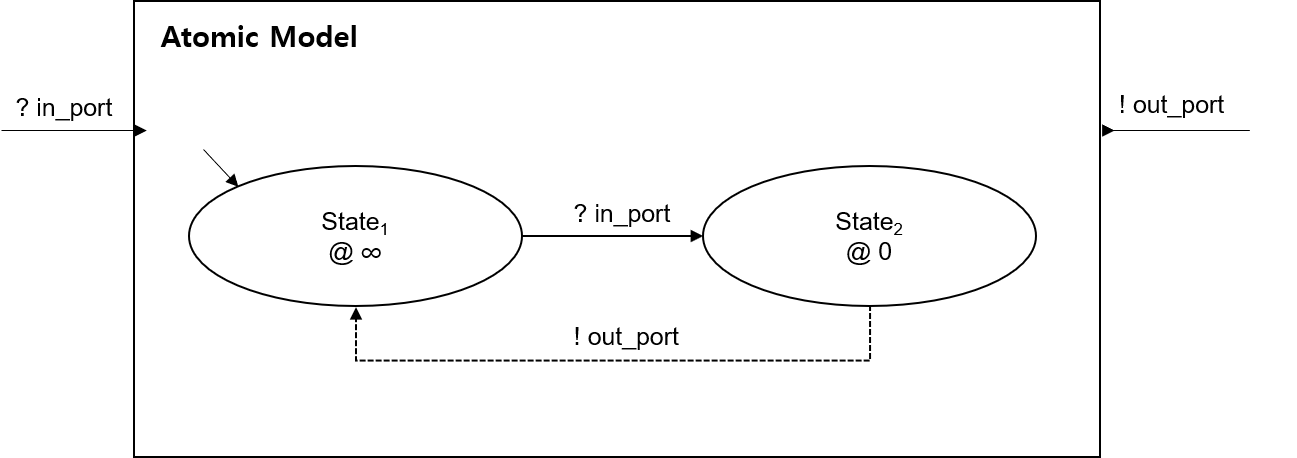
\includegraphics[width=1.0\columnwidth]{fig/Atomic_model}
    \caption{Example of an Atomic Model}
    \label{Fig:AtomicModel}
\end{figure}

Figure~\ref{Fig:AtomicModel} shows the diagram of an Atomic Model.~The label starting with the question mark denotes the input port, and the label starting with the exclamation mark denotes the output port.~The ellipse shows the state of the model and ellipse with an arrow denotes the initial state of the model.~Each state has the state name and the positive real number which denotes the occupancy time.~When the elapsed time meets the occupancy time, the simulation algorithm will trigger the output function and internal transition function, sequentially. 

The proposed simulator partially accepts the notation of DEVS formalism and its simulation algorithm.~Listing~\ref{lst:atomic} shows the python code of the example atomic model.~As shown in the Listing~\ref{lst:atomic}, the proposed simulator provides a programming interface that has a one-to-one correspondence with the Atomic Model specification of the DEVS formalism.


\begin{lstlisting}[language=Python, caption=Example Code of Atomic Model, label={lst:atomic}]
class AtomicModel(BehaviorModelExecutor):
    def __init__(self, instance_time, destruct_time, name, engine_name):
        BehaviorModelExecutor.__init__(self, instance_time, destruct_time, name, engine_name)

        self.init_state("State1")
        self.insert_state("State1", Infinite)
        self.insert_state("State2", 0)

        self.insert_input_port("in_port")
        self.insert_output_port("out_port")

    def ext_trans(self,port, msg):
        if port == "in_port":
            self._cur_state = "State2"

    def output(self):
        name = self.get_name()
        msg = SysMessage(name, "out_port")
        return msg
        
    def int_trans(self):
        if self._cur_state == "State2":
            self._cur_state = "State1"
\end{lstlisting}

\section{Proposed Method and Environments}

This section introduces the modeling results of simulation entities of the municipal solid waste management system and its simulation environment. This research proposes two modeling methods to model the municipal waste management system; First, we separate the domain related part and the simulation related part. Second, we adopt the object-oriented concept so that the simulationists may select simulation entities and synthesize the simulation based on the target situations. Therefore, experts with various levels of understanding may participate in simulation development and experiments.

To capture the dynamic behavior of the residents, we classified the type of residents and modeled the residents using DEVS formalism. The parameters required for a simulation are modeled as a class definition in Python programming language. Also, simulation entities that modeled as an Atomic Model inherit the base class for discrete event simulation. Each class instance of the resident type and a discrete event simulation model are synthesized during the initialization phase of the simulation. 

Following Listing~\ref{lst:domain} shows the example code of the resident class for a student. The code returns information of a resident as wake up time, sleep time,  and the amount of waste discharge. Each information is based on the survey of "What time did you wake up today?" conducted by Gallup Korea in 2013~\cite{gallup2013}. 

\begin{lstlisting}[language=Python, caption=Example Code of Resident for Student, label={lst:domain}]
class Student(HumanType):
    def __init__(self,_id):
        HumanType.__init__(self ,_id)
        pass
    
    def get_type(self):
        return "Student"

    def get_wakeup(self):
        return TimeStruct(7,58, Statistic(0, 0, 1))
        
    def get_sleep(self):
        return TimeStruct(24,51, Statistic(0, 0, 1))
  
    def get_out(self):
        return self.get_wakeup() + 1

    def get_in(self):
        return TimeStruct(21,00, Statistic(0, 0, 1))

    def get_trash(self):
        return 0.3        

    def get_satisfaction_func(self, trash):
        if trash >= 0.8 :
            return -10
        elif trash <= 0:
            return 20
        elif trash < 0.8:
            return 10
\end{lstlisting}

\begin{figure*}[ht]
    \centering
    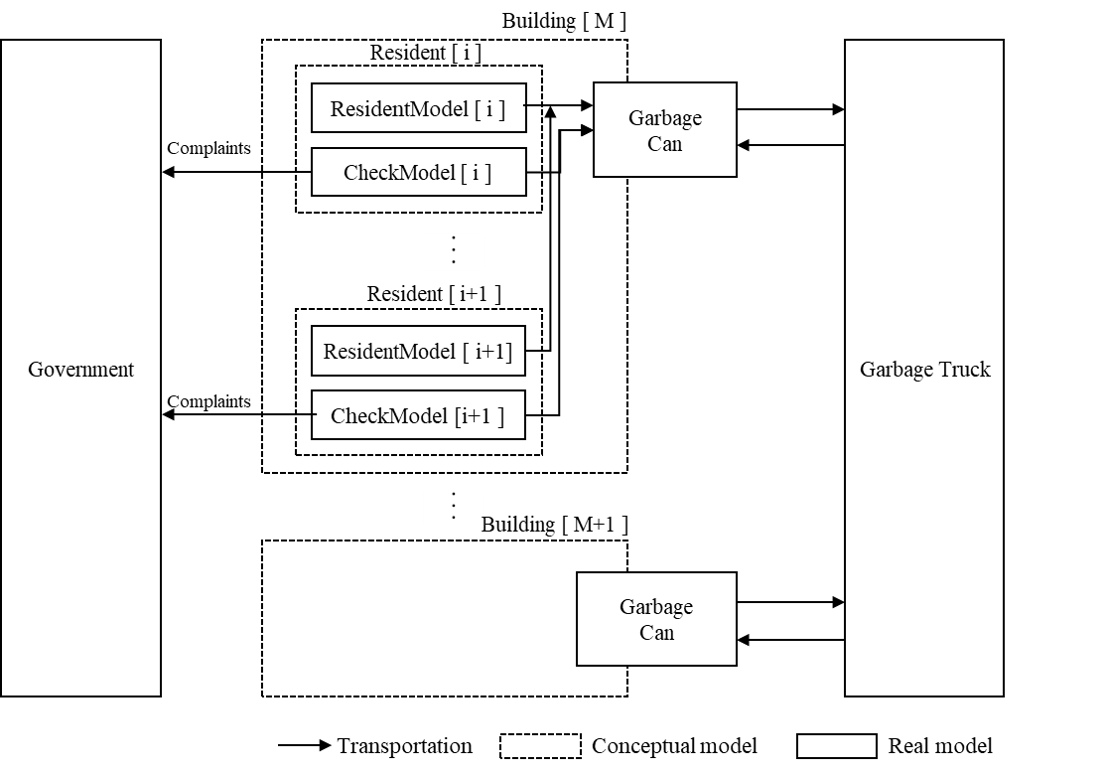
\includegraphics[width=1.5\columnwidth]{fig/framework_revised}
    \caption{Atomic Model to Calculate the Satisfaction Level of a Resident}
    \label{Fig:Framework}
\end{figure*}

Figure~\ref{Fig:Framework} shows the overall framework of the proposed simulation environment.~The urban planner may compose the simulation models to represent the residential areas by connecting the ports to the other simulation models' port.

Figure~\ref{Fig:residentmodel} shows the diagram of a Resident Model to model the residential area. The Resident Model may calculate the leave time based on the wake time of a resident type instance, as shown in \ref{lst:domain}. Therefore, the simulationists may reuse the Resident Model by changing the resident type instance objects. Moreover, this research takes normal distribution for the given leave time for stochastic simulation. During the simulation, the Resident Model may generate a trash event with a given amount of waste discharge from a resident type instance and send to their family model and check model. 

\begin{figure}[!ht]
    \centering
    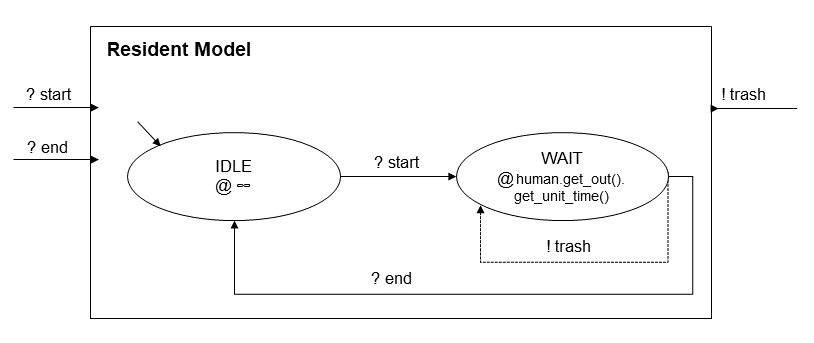
\includegraphics[width=1.0\columnwidth]{fig/resident_model.jpg}
    \caption{Atomic Model of a Resident}
    \label{Fig:residentmodel}
\end{figure}


%\begin{figure}[!ht]
%    \centering
%    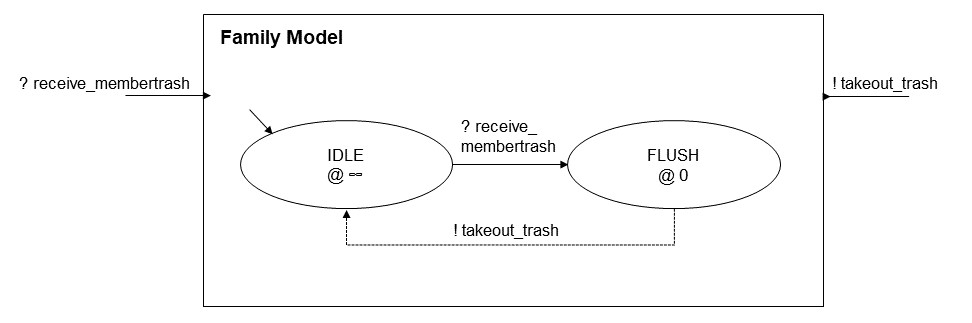
\includegraphics[width=1.0\columnwidth]{fig/family_model.jpg}
%    \caption{Atomic Model of a Housing Type}
%    \label{Fig:Familymodel}
%\end{figure}

%Figure~\ref{Fig:Familymodel} shows the diagram of a Family Model.~Family models are a set of resident models. We created a family model to implement the actual furniture and randomly linked residents to the family model.~Depending on the number of families, each family's garbage storage size and the $Leave\ time$ will vary.~Receive garbage data from the resident model through the receive-membertrash port and add it to the current storage size.~If the current storage size is larger than the garbage storage size, one random member of the family was selected to take out trash based on the $Leave\ time$ of the selected person.~Transfer current storage size to the garbage can model through the takeout-trash port and change the current storage size to 0.

\begin{figure}[!ht]
    \centering
    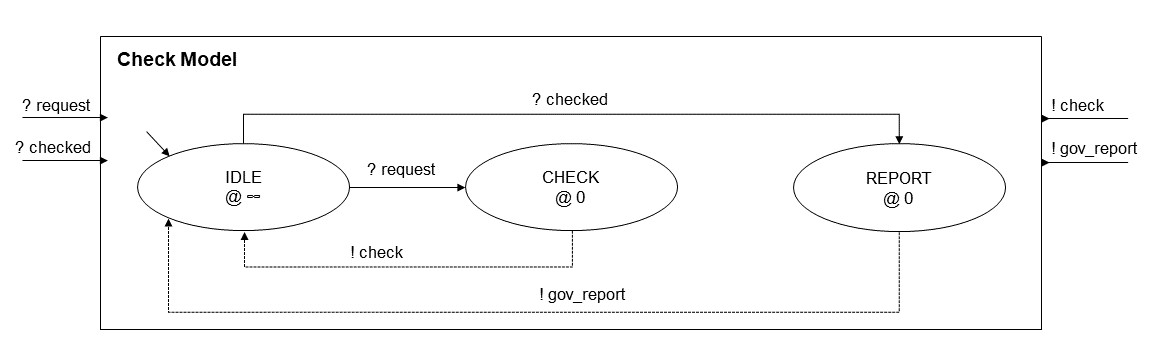
\includegraphics[width=1.0\columnwidth]{fig/check_model.jpg}
    \caption{Atomic Model to Check the garbage}
    \label{Fig:Checkmodel}
\end{figure}

Figure~\ref{Fig:Checkmodel} shows the diagram of a Check Model.~This is the measurement model for the satisfaction level of residents according to the capacity of the garbage can. Since most residents do not check the trash during the daytime, the Check Model checks the garbage can at the leave time of a resident. Therefore, the check model checks the garbage-can periodically on the leave event. Since the Resident Model send the trash event based on the leave time, the check model utilizes the event to handle the leave event. As a result, the satisfaction level of a resident with the cleanliness of the garbage collection site is measured every leave time. When the Check Model receives a request message from the Resident model, a check message is sent to the garbage can model to check the status of the garbage can. If the value received from the garbage-can through the check port, the check model passes the value to the resident type instance. Each resident type class has a function that calculates the satisfaction level based on the accumulation ratio of garbage-can. After checking the satisfaction level, the check model may trigger, claim message to the Government Model through the gov-report port, if the satisfaction level goes under the threshold.

\begin{figure}[!ht]
    \centering
    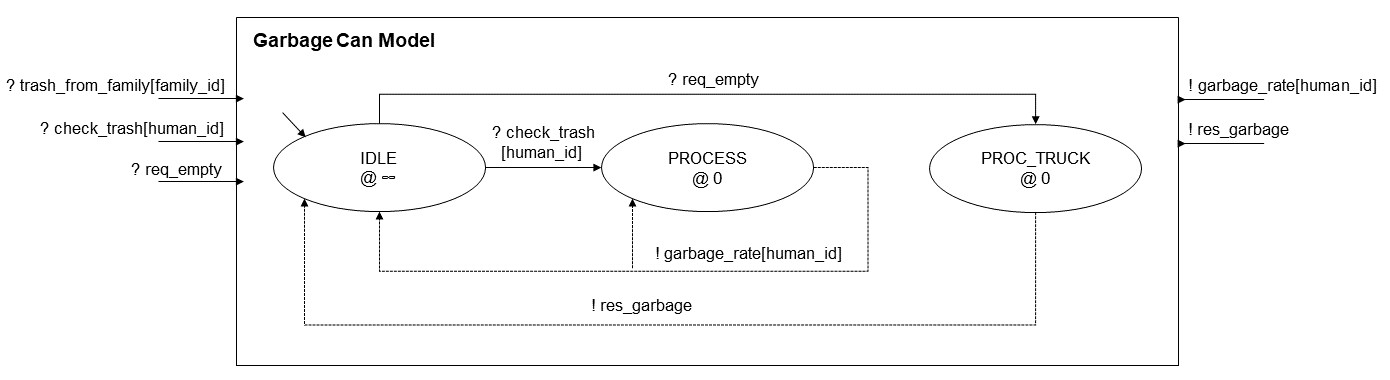
\includegraphics[width=1.0\columnwidth]{fig/garbagecan_model.jpg}
    \caption{Atomic Model to Calculate the garbage of a Building}
    \label{Fig:Garbagemodel}
\end{figure}

Figure~\ref{Fig:Garbagemodel} shows the diagram of a GarbageCan Model. The GarbageCan model models the temporary garbage collection area for each building. Each GarbageCan model may have different free space during the simulation. If residents discharge a large amount of garbage to the garbage-can or a garbage truck did not collect the enough garbage from the garbage-can, the garbage-can may have remain garbage. The remaining garbage may affect the satisfaction level of a resident. Therefore, a simulationist may observe changes in the residents' satisfaction according to the capacity of the garbage can and estimate the capacity of the proper garbage's size according to the residents. 
When a GarbageCan model receives an event from the $trash_from_family port$, the GarbageCan is filled with garbage with the given value. Also, when the GarbageCan model receives the event from the Check Model, the GarbageCan calculates the accumulation ratio of the garbage-can and sent back to the Check Model. Finally, when the GarbageCan model receives a message from the Garbagetruck Model, the accumulated amount of garbage is sent to the Garbagetruck Model.

\begin{figure}[!ht]
    \centering
    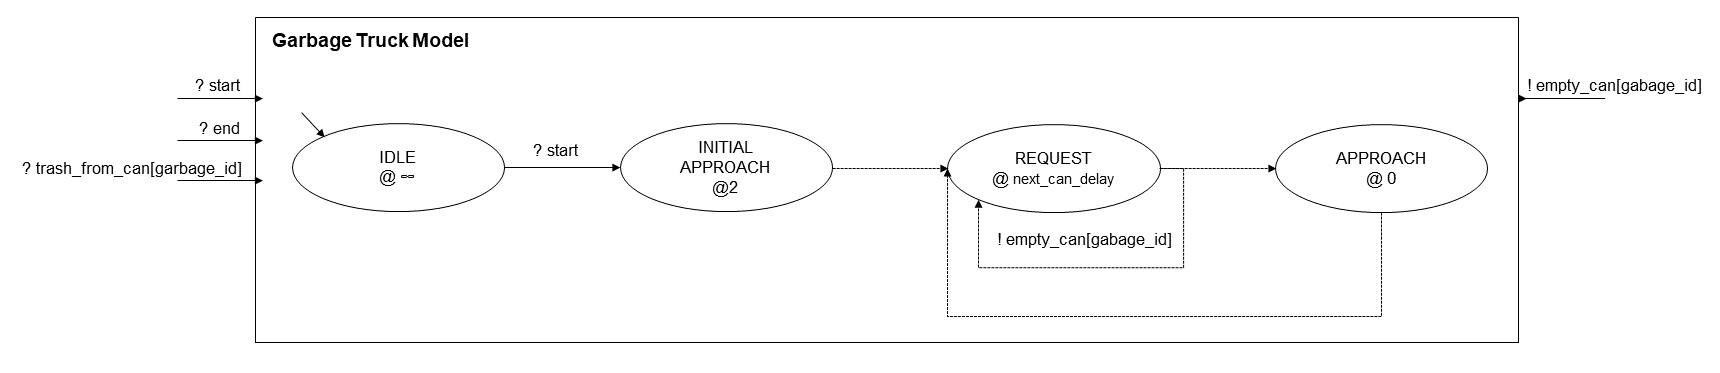
\includegraphics[width=1.0\columnwidth]{fig/garbagetruck_model.jpg}
    \caption{Atomic Model to Collect the garbage in a building}
    \label{Fig:garbageTruckmodel}
\end{figure}

Figure~\ref{Fig:garbageTruckmodel} shows the diagram of a GarbageTruck Model.~This model is designed to retrieve garbage from buildings at regular intervals.~The parameters of the GarbageTruck model are the visit order of the buildings, the collection time for each building, the capacity of the garbage truck, and the collection cycle. Each parameter can be adjusted to create an optimized waste management system. 
When the GarbageTruck model visits the building, the truck takes the garbage from the garbage-can and add the garbage to the truck. The truck has fixed size storage so that the amount of garbage cannot exceed the storage of a truck. Therefore, GarbageTruck may not collect the garbage from the GarbageCan when the truck does not have enough storage. 
The GarbageTruck model sends a message to receive the accumulated garbage from a GarbageCan. This process is repeated until the truck visits all buildings. After visiting all buildings, the amount of storage for a truck set to zero and reschedule the garbage collection. 

\begin{figure}[!ht]
    \centering
    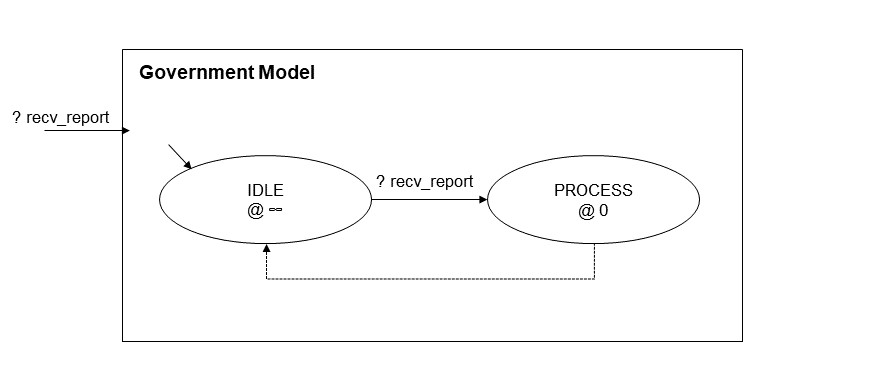
\includegraphics[width=1.0\columnwidth]{fig/government_model.jpg}
    \caption{Atomic Model to Receive report from Resident}
    \label{Fig:Governmentmodel}
\end{figure}

Figure~\ref{Fig:Governmentmodel} shows the diagram of a Government Model.~The Government Model collects complaints from the residents. To help simulationists, the model records the complaints period and satisfaction level of a resident. 

% 모델링을 어떻게 했다. 
% 사람, 직업, 행위에 대해서 모델링을 어떻게 했다고 작성

%우리가 하려는 것들
%Behaviourmodel, Familymodel, garbagecan, garbagetruck, checker 등등 
%상속 하는 그림,
%각 모델에서 설명 (human - 직업)
%직업이 simulation에 영향을 줌 -> 직업별 행동패턴을 부여해서 모델링 하는게 좋다
%Report하는 사람과 안하는 사람 리스트나 튜플 형태로 표현


\section{Case Study}
This section illustrates the case study of the proposed method and the simulation environments.~Based on the population composition of an administrative district in Pohang City, Republic of Korea, an experiment was conducted by modeling the life patterns of construction workers, students, and housewives, who occupy the majority of the administrative districts. The life pattern for each job was based on the analysis data \cite{gallup2013} of a public opinion survey institute targeting the national population and used data on the time to work and the amount of garbage discharged.
\subsection{Modeling}
As for the actual operation of garbage collection vehicles, the situation may be different for each garbage disposal company. Also, to clearly show individual patterns, every household was set as a single-person household.
\subsubsection{agent}
%? %

\subsubsection{building}
There are a total of 33 people in one building, and three buildings are modeled. There is one trash can for each building.
\subsubsection{garbage truck}
Garbage truck collects trash from the garbage can of each building as much as the remaining capacity of the truck. Collection time was set based on an hour before and after each job's average time to go to work. In the case of daily workers, their leaving time was earlier than the city's designated starting time for garbage collection, so the time before and after construction workers go to work was not taken into account.
\begin{figure}
  \centering
    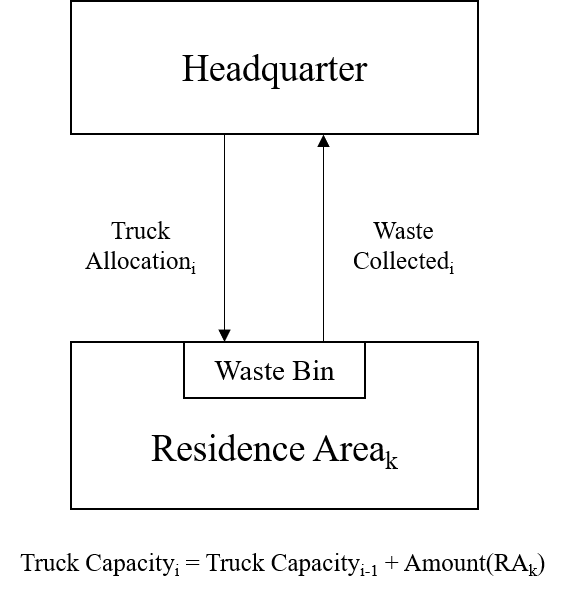
\includegraphics[width=.80\columnwidth]{fig/HQTruckCapacity.png}
    \caption{Truck Capacity}
    \label{Fig:Truck Capacity}

\end{figure}
%pattern 에 대한 설명
The fixed sequence refers to the sequence that repeats one cycle of collection. For example, if there are 3 buildings; building A, B, and C. When the garbage truck visits the building in alphabetical order, one cycle of schedule would be A->B->C. In a fixed sequence, "A->B->C" cycle would be repeated. The palindrome sequence refers to the sequence that reverses the order after finishing each cycle of collection. In a palindrome sequence, the garbage truck visits the last building for the first in the next cycle, and the building visited for the first in the previous cycle would be visited for the last(A->B->C->C->B->A). Lastly, the random sequence refers to visiting every building at random order.

\subsection{Simulation}
Simulation environment
CPU Intel Core i7-7700K @ 4.20GHZ
RAM 64GB
GPU NVIDIA GeForce GTX1080
%Took 5min 30s for each scenario. @timefn: execute_fn took %333.8098875639989 seconds           
In the experiment, the average number of complaints of the residents was measured by simulating 30 times by changing the random seed for the fixed sequence, the palindrome sequence, and the random sequence.


%\end{itemize}


\begin{comment}
\begin{figure}[!ht]
    \centering
    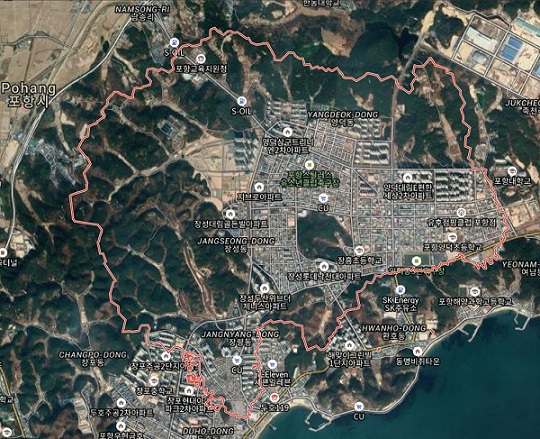
\includegraphics[width=1.0\columnwidth]{fig/map.jpg}
    \caption{Map of Jangryang-dong, Pohang represented within the red bold lines}
    \label{Fig:JangYrang}
\end{figure}
\end{comment}
\subsubsection{Assumptions and the Simulation Parameter}

The following are assumptions made for modeling the general case.
\begin{itemize}
    \item Each building has a garbage can to hold the garbage temporarily.
    \item Each resident has their own schedule to go out.
    \item Every resident takes out garbage every day when they go out. 
    \item The satisfaction level of the resident may change at the moment when resident take out the garbage.
    \item The resident may complain to the Government when the garbage goes above a certain level.
\end{itemize}

\begin{table*}[ht]
\centering
\small
\caption{Description of Simulation Parameters}
\begin{tabular}{|l|c|c|c|}
\hline
 & Construction Worker & Student &Housewife \\ \hline
Leave Time & 6:22:00 & 7:58:00  & 13:00:00\\ \hline
Amount of Waste Discharge & 0.9& 0.9& 0.9\\ \hline
Satisfaction Function & 
    $Sat(x) = \begin{cases}
              + 10 & \text{if } x < 0.8,\\
              \ \ \ 20 & \text{if } x = 0,\\
               -10 & \text{if } x > 0.8
          \end{cases}$
 & $Sat(x) = \begin{cases}
              + 10 & \text{if } x < 0.8,\\
              \ \ \ 20 & \text{if } x = 0,\\
               -10 & \text{if } x > 0.8
          \end{cases}$
          & $Sat(x) = \begin{cases}
              + 10 & \text{if } x < 0.8,\\
              \ \ \ 20 & \text{if } x = 0,\\
               -10 & \text{if } x > 0.8
          \end{cases}$ \\ \hline
\end{tabular}
\label{tab:SimParam}
\end{table*}
Following Table~\ref{tab:SimParam} shows the simulation parameters deduced from the assumptions.~$Leave\ Time$ represents an interval at which one leaves one's home.~We modified the $Leave\ time$ based on average wake-up time data from living time survey~\cite{gallup2013}.~$Amount\ of\ Waste\ Discharge$ represents the amount of waste generated until out time. For realistic simulation, The amount of waste generation of the residents is drawn from average waste discharge per capita~\cite{Korea_resource_recirculation_information_system_2018}.~$Satisfaction\ Function$ represents one's satisfaction level according to the level of garbage. Based on the experiences of some students, the decision made by the heuristic.

% 이상의 파라미터 값이 어떻게 책정되었는지가 설명되어야 함


\subsection{Lesson Learned}

\begin{figure}[!h]
    \centering
    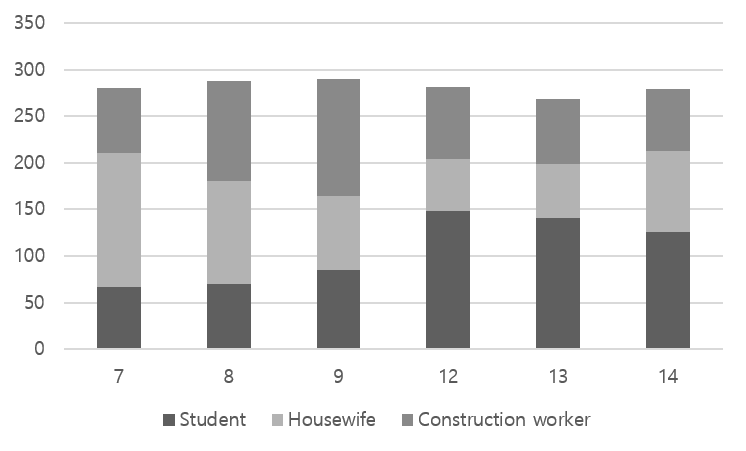
\includegraphics[width=1.0\columnwidth]{experiment_result/FixedSequence.png}
    \caption{Fixed Sequence}
    \label{Fig:Fixed Sequence}
\end{figure}
\begin{figure}[!h]
    \centering
    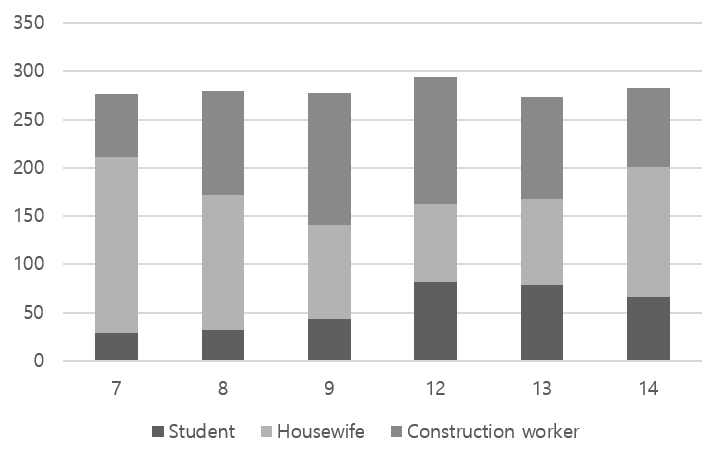
\includegraphics[width=1.0\columnwidth]{experiment_result/withmultipleHousewife.png}
    \caption{Fixed Sequence with Multiple Housewife}
    \label{Fig:Fixed Sequence with Multiple Housewife}
\end{figure}
\begin{figure}[!h]
    \centering
    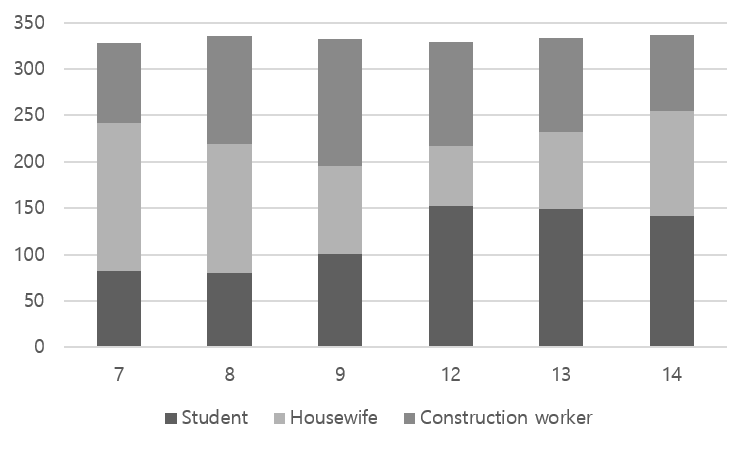
\includegraphics[width=1.0\columnwidth]{experiment_result/PalindromeSequence.png}
    \caption{Palindrome Sequence}
    \label{Fig:Palindrome Sequence}
\end{figure}
\begin{figure}[!h]
    \centering
    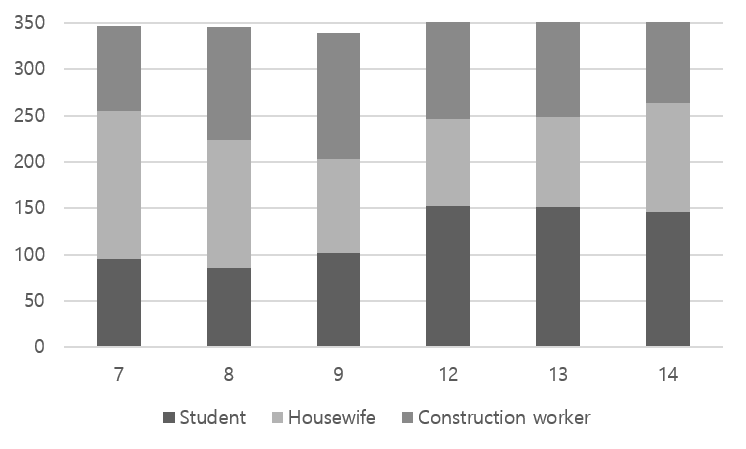
\includegraphics[width=1.0\columnwidth]{experiment_result/RandomSequence.png}
    \caption{Random Sequence}
    \label{Fig:Random Sequence}
\end{figure}

\section{Conclusion}
\begin{comment}	
주거민의 행동패턴을 기반으로 한 도시 모델링 및 시뮬레이션의 중요성
주거민 행동패턴을 기반으로 한 모델링 시뮬레이션 환경을 구축하였다.
\end{comment}
As the complexity of an urban area increases, estimating waste generation and providing an alternative solution for waste collection are important for urban planners and employees of the local government to increase the satisfaction level of residents.To compute the approximated satisfaction level of residents, this research modeled the residents' life patterns and housing types to estimate waste generation and collection. The proposed modeling and simulation environment was modeled on the agent, building, garbage truck and operation strategy based on DEVS formalism. In this environment, various assumptions and operation strategies were established and tested. The results of the experiment showed that the number of complaints may vary depending on the population composition ratio, and the number of complaints was the lowest when collecting at 1:00 PM independent of the population composition in a fixed sequence collection with a given experimental environment. Therefore, it is possible to perform modeling on the population composition and residential area of the actual city and set the optimal collection time according to the existing collection pattern. Alternatively, the proposed modeling and simulation environment and alternative derivation methods can be used to derive the optimal collection pattern. For the future research, an experiment can be conducted on a family-unit waste discharge pattern with 1 person household, 2 person household or 3 person household. In addition, experiment of validating effectiveness of installing smart garbage can be done  If local governments can deploy the IOT trash cans to find out the amount of garbage discharged, how much complaints will be reduced when dynamic vehicle routing become available. Implementing a graphical user interface to increase the usability to urban planners or the employees of the local government can be also considered.


For the future research guideline, attaching GIS to reflect the real-world data or 



\balance

\bibliographystyle{unsrt}
\bibliography{References}

\end{document}
